% To je predloga za poročila o domačih nalogah pri predmetih, katerih
% nosilec je Blaž Zupan. Seveda lahko tudi dodaš kakšen nov, zanimiv
% in uporaben element, ki ga v tej predlogi (še) ni. Več o LaTeX-u izveš na
% spletu, na primer na http://tobi.oetiker.ch/lshort/lshort.pdf.
%
% To predlogo lahko spremeniš v PDF dokument s pomočjo programa
% pdflatex, ki je del standardne instalacije LaTeX programov.

\documentclass[a4paper,11pt]{article}
\usepackage{a4wide}
\usepackage{fullpage}
\usepackage[utf8x]{inputenc}
\usepackage[slovene]{babel}
\selectlanguage{slovene}
\usepackage[toc,page]{appendix}
\usepackage[pdftex]{graphicx} % za slike
\usepackage{setspace}
\usepackage{color}
\definecolor{light-gray}{gray}{0.95}
\usepackage{listings} % za vključevanje kode
\usepackage{hyperref}
\usepackage{float}
\usepackage{verbatim}
\renewcommand{\baselinestretch}{1.2} % za boljšo berljivost večji razmak
\renewcommand{\appendixpagename}{Priloge}

\lstset{ % nastavitve za izpis kode, sem lahko tudi kaj dodaš/spremeniš
language=Python,
basicstyle=\footnotesize,
basicstyle=\ttfamily\footnotesize\setstretch{1},
backgroundcolor=\color{light-gray},
}

\title{Peta domača naloga}
\author{Anže Pečar (63060257)}
\date{\today}

\begin{document}

\maketitle

\section{Uvod}

Cilj domače naloge je bil seznaniti se z linearno regresijo.
\section{Podatki}

Za podatke sem "zelel uporabiti bazo podatkov o pogodbah podjetja pri katerem ob"casno delam. Pridobil sem si dovoljenje za uporabo teh podatkov, vendar so se na "zalost izkazali za neprimerne, saj nobeni atributi niso bili medsebojno odvisno. "Se najbolje je kazalo atributu "st. obrokov in razredom znesek pogodbe, vendar kot je razvidno iz slike \ref{pogodbe} ni nobene lepe povezanosti.

\begin{figure}[H]
\begin{center}
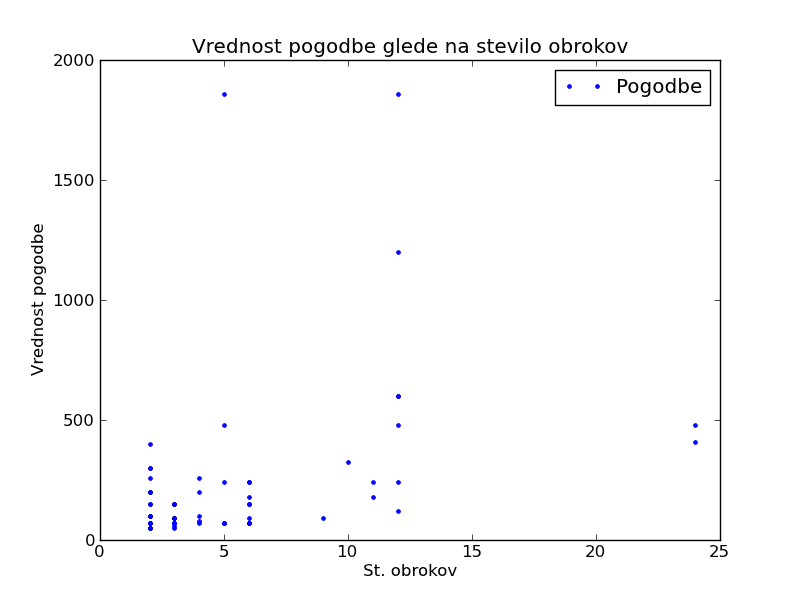
\includegraphics[scale=0.3]{pogodbe.png}
\caption{Znesek pogodbe v odvisnosti od "st. obrokov}

\end{center}
\label{pogodbe}
\end{figure}

Zato sem na koncu uporabil podatke iz online ml te"caja, prikaz podatkov je na sliki \ref{mldata}.

\begin{figure}[H]
\begin{center}
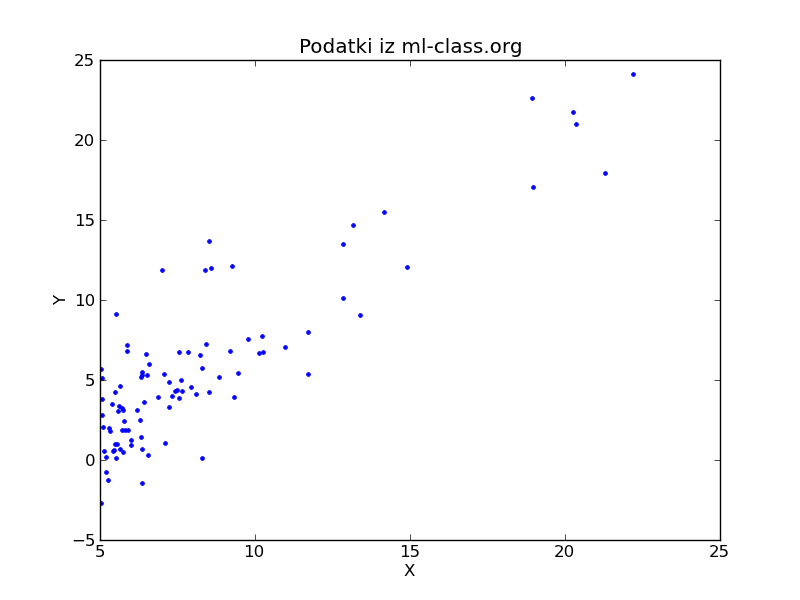
\includegraphics[scale=0.3]{ml-data.png}
\caption{Podatki iz ml-class.org}
\end{center}
\label{mldata}
\end{figure}

\section{Rezultati}
\subsection{Prva to"cka}
\subsection{Druga to"cka}
\subsection{Tretja to"cka}

%\begin{table}[H]
%\caption{Oddaje}
%\begin{tabular}{ c | c | c | c | c | p{6cm} }
%  & Ime metode & Oddaja & ocena F &  F & Komentar\\
%  \hline \hline
%  * & 1R & 07.03. 13:31:56 & 0.33735 & 0.33878 & 1R s štetjem atributov \\ \hline
%  * & 1RS &09.03. 09:18:21 & 0.36952 & 0.36384 & 1R s seštevamjem vrednosti atributov \\\hline
%  * & RF &10.03. 09:44:08 & 0.38073 & 0.40977 & 250 dreves, prag 0.20, max 6 napovedanih razredov \\ \hline
%  * & RF &11.03. 08:09:49 & 0.37891 & 0.40387 & 500 dreves, prag 0.20, max 6 napovedanih razredov \\ \hline
%  & RFN &17.03. 16:02:10 & 0.38635 & 0.41439 & 500 dreves, normaliziran prag 0.5 \\ 
%\hline
%  & RFN &17.03. 23:29:35 & 0.38235 & 0.40337 & 500 dreves, normaliziran prag 0.1921 \\ \hline
%
%  & RFDP &18.03. 12:53:21 & 0.39655 & 0.43659 & 500 dreves, dinamični prag 0.221 \\ 
% \end{tabular}
% \label{tabela}
%\end{table}

%\begin{figure}[H]
%\begin{center}
%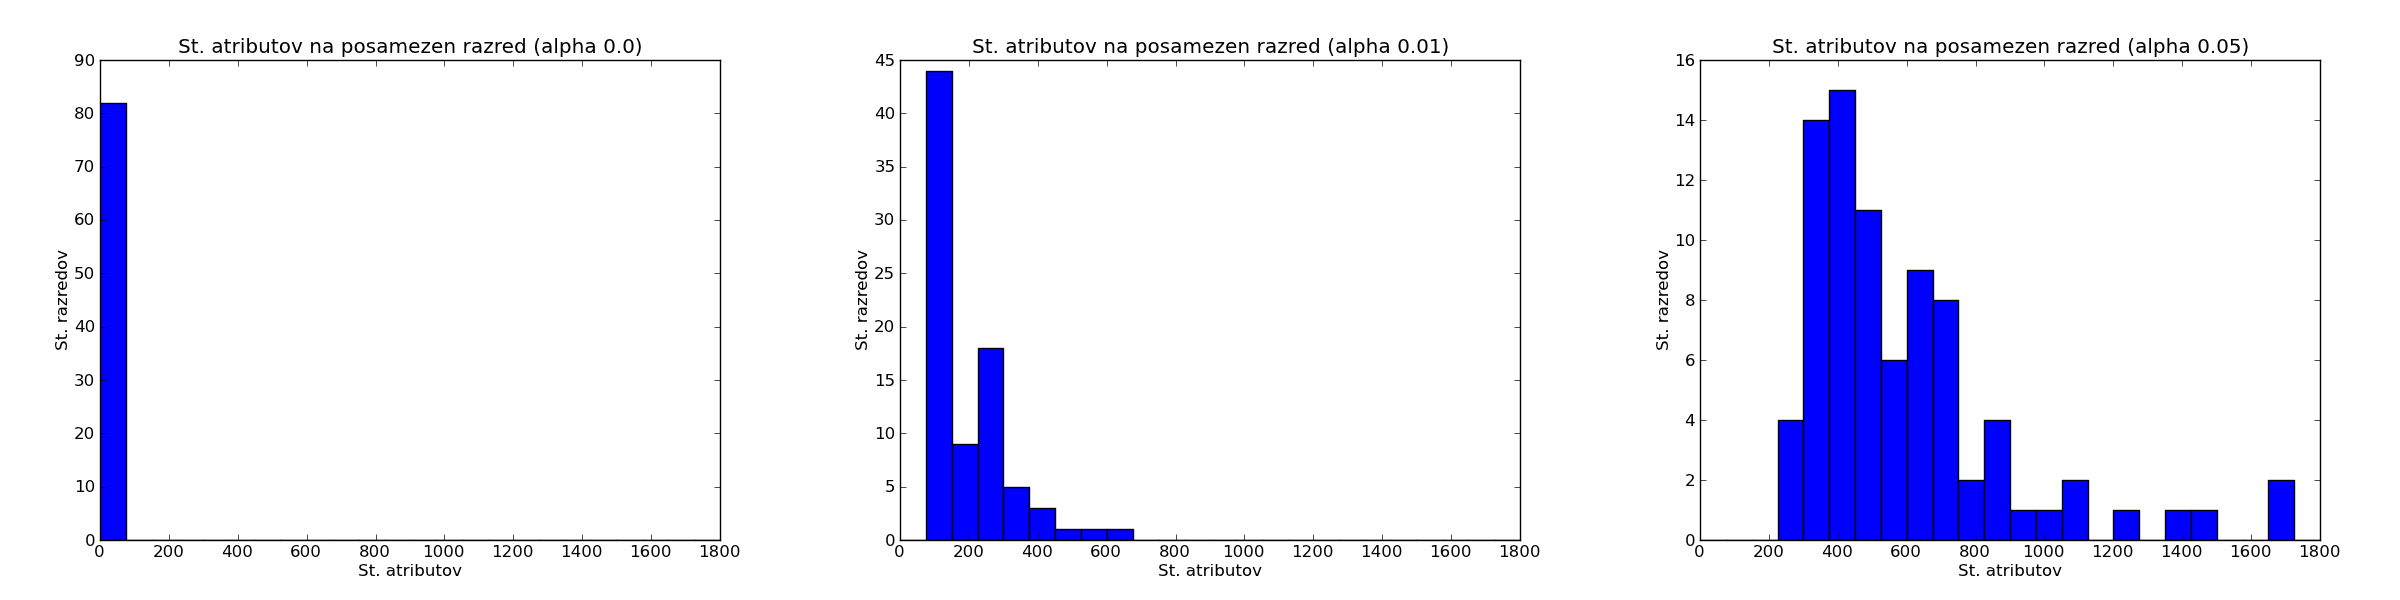
\includegraphics[scale=0.2]{skupno100.png}
%\caption{Rezultati 100 permutacij za različne vrednosti Alpha}
%\label{skupno100}
%\end{center}
%\end{figure}

\section{Izjava o izdelavi domače naloge}
Domačo nalogo in pripadajoče programe sem izdelal sam.


\begin{thebibliography}{9}

\bibitem{mining}
   Ian H. Witten \& Eibe Frank,
   \emph{Data Mining Practical Machine Learning Tools and Techniques, Second Edition}
   Morgan Kaufmann Publishers,  
   2005.

\end{thebibliography}

\end{document}
